%&latex
\documentclass[msc, openright, a4paper]{TNthesis}

%package declaration 
\usepackage{times}
\usepackage{paralist}
\usepackage{graphicx}
\usepackage{indent}  
\usepackage{listings} 
\usepackage{rotating}
\usepackage{bnf}
\usepackage{color} 

\author{Galiia Khasanova}

\newcommand\B{\rule[-1.7ex]{0pt}{0pt}} % Adds a space between the text and the [B]ottom \hline
\newcommand\T{\rule{0pt}{3.1ex}} % Adds a space between the text and the [T]op \hline

\enlargethispage{5cm} \thispagestyle{empty} \vsize=25.0cm

\abstract{
 This thesis presents blah blah blah.
 }
\begin{document} 


\begin{preliminary}

\begin{titlepage}
	    \begin{center}
	    \vspace{-7.3cm}
	    
\includegraphics[scale=.6,width=12.5cm]{img/logo_eumi.eps}\\
	%
	 \vspace{0.3cm}
	        \begin{LARGE}
	        UNIVERSIT\`A DEGLI STUDI DI TRENTO
	        \end{LARGE}\\
	    \begin{large}
	        Facolt\`a di Scienze Matematiche, Fisiche e Naturali\\
	    \end{large}
	        \ \\
	    \vspace{0.5cm}
	    
\includegraphics[width=2.5cm]{img/logo_unitn.eps}\\
	    \vspace{-0.3cm}
	    \begin{Large}
	        \ \\
	        Corso di Laurea Specialistica in Informatica\\
	        Within European Masters in Informatics
	        \end{Large}
	        \ \\
	        \hrule
	        \ \\
	        \begin{Large}
	        Tesi di Laurea\\
	        \end{Large}
	        \vspace{1.0cm}
	    \begin{center}
	    \begin{LARGE}
	        \textbf{High Level Programming of Wireless Sensor Networks Using Distributed Abstract Data Types}\\
	        \end{LARGE}
	    \end{center}
	
	        \vspace{1.2cm}
	    \end{center}
	\begin{center}
	    \begin{tabular}{ll}
	        \large{Relatori} & \hspace{5 cm} \large{Laureanda}\\
	        \small{\ } & \small{ }\\
	        \large{\textbf{Gian Pietro Picco}} & \hspace{5 cm}
	        								\large{\textbf{Galiia Khasanova}}\\
	        \large{\textbf{Klaus Wehrle}} & \hspace{5 cm}\\
	    \end{tabular}
	\end{center}
	    \vspace{1.3cm}
	    \begin{center}\begin{large}Anno accademico 2007/2008\end{large}\end{center}
\end{titlepage}

\standarddeclaration

\begin{acknowledgements}
	Bla
\end{acknowledgements}

\begin{acronyms}
	\begin{center}
	\begin{tabular}{| l |p{9cm}|}
	\hline
	ADT \T \B & Abstract Data Type \\
	\hline
	CLDC \T \B & Connected Limited Device Configuration \\
	\hline
	DADT \T \B & Distributed Abstract Data Type \\
	\hline
	Java ME \T \B & Java Micro Edition \\
	\hline
	JiST \T \B & Java in Simulation Time \\
	\hline
	JVM \T \B & Java Virtual Machine \\
	\hline 
	LN \T \B & Logical Neighborhoods \\
	\hline
	MAC \T \B & Media Access Control \\
	\hline
	MEMS \T \B & Micro-Electro-Mechanical Systems \\
	\hline
	OS \T \B & Operating System \\
	\hline
	QoS \T \B & Quality of Service \\
	\hline
	RF \T \B & Radio Frequency \\
	\hline
	Sun SPOT \T \B & Sun Small Programable Object Technology \\
	\hline
	SWANS \T \B & Scalable Wireless Ad hoc Network Simulator \\
	\hline
	VM \T \B & Virtual Machine \\
	\hline
	WSN \T \B & Wireless Sensor Network \\
	\hline
	WSAN \T \B & Wireless Sensor and Actor Networks \\
	\hline
	\end{tabular}
	\end{center}
\end{acronyms}


%\dedication{To Eric Cartman, Southpark, Colorado, USA. Only because my
%boyfriend insists.}
\tableofcontents
\listoffigures
%\listoftables
\end{preliminary} 


\chapter{Introduction}

\textcolor{green}{Jo: quote is fine, but better Sth Like : Mark Weiser once
wrote in his visionary paper from whenever [22]:}

\begin{quote}
\emph{``The most profound technologies are those that disappear. They weave
themselves into the fabric of everyday life until they are indistinguishable
from it''} 
Mark Weiser \cite{Weiser_ComputerIn21stCentury}
\end{quote}


\textcolor{blue}{some intro words here.. .. and later stuff about .. The chapter
begins with an introduction to wireless sensor nodes and Wireless Sensor Networks (WSNs). This is followed by a
description of the protocol stack used in this work}



\section{Introduction to Wireless Sensor Networks}

Recent advances in micro system technologies and wireless communication
made it possible to deploy wireless sensor networks (WSNs) that contain a large
number of sensor nodes, multifunctional devices characterised by their low- cost,
low-power, and small form factor, that can communicate across short distances
using Radio Frequency (RF) communication \cite{SensorSurveyAkyildiz:2002}.

WSNs are being used in a wide range of applications in military and civilian
operations such as, for instance, health monitoring, environment monitoring,
data acquisition in dangerous environments, and target tracking.

This chapter begins with the introduction of sensor nodes and
discussion over followed by presentation of the most important features of WSNs.

\subsection{Sensor Nodes} \label{subsec:sensornodes}

Typically, a sensor node consists of the following elemants (as it can be seen
from the Figure \ref{Fig:SensorNodeArch})
\begin{itemize}
  \item \emph{Sensing unit}, which is comprised of a number of sensors and
  analog-to-digital converters. 
  \item \emph{Tranceiver}, which facilitates node-node communication using 
a variety of techniques.
  \item \emph{Processing unit}, that usually comprises a 
microcontroller/microprocessor that performs processing, and is associated with 
a storage unit.
  \item \emph{Power unit}, which provides the energy required to run the sensor node, and can use chemical 
batteries or power scavenging units such as solar cells.
\end{itemize}


\begin{figure}
\centering
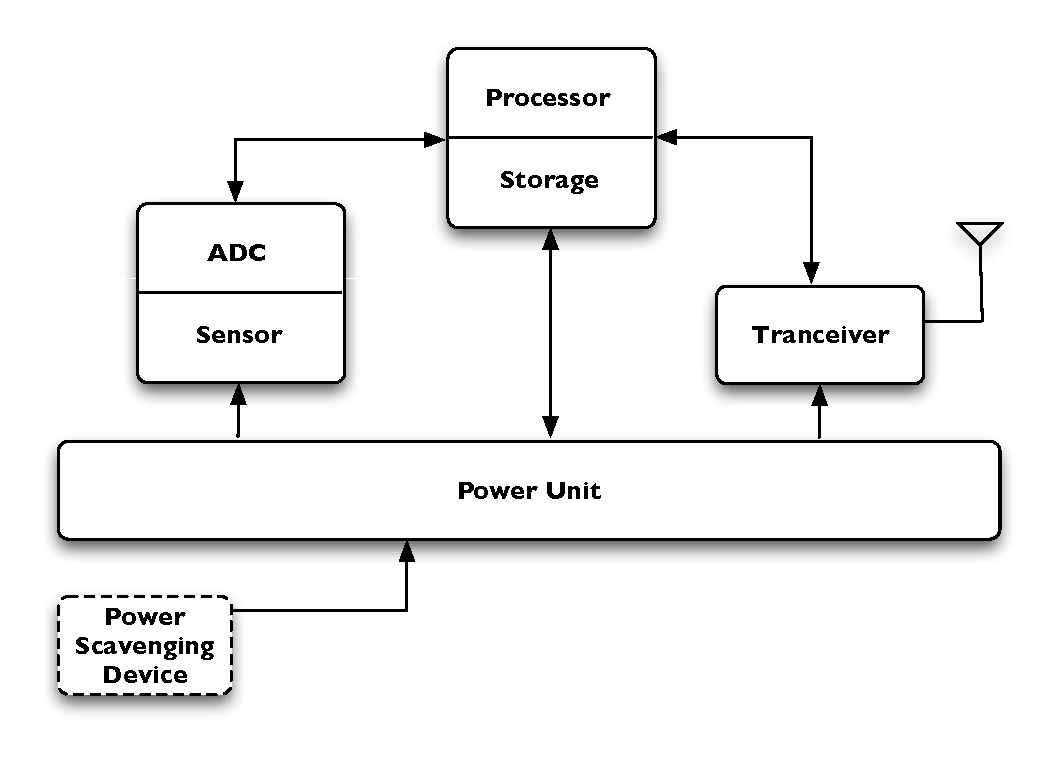
\includegraphics[scale=0.65]{img/SensorNodeArch.eps} 
\caption[Architecture of a sensor node] {Architecture of a sensor node (adapted from \cite{SensorSurveyAkyildiz:2002}).}
\label{Fig:SensorNodeArch}
\end{figure} 


\textcolor{green}{the next paragraph needs a bit of reformulation. about the constraints
I think your argumentation should go like size/weight -> battery  (that's the
point where it really gets hard to make smaller). -> energy efficient processing, memory and so on
and cost as an additional constraint }

Sensor nodes have constraints on both their size and their cost. The former 
constraint arises from the requirement that sensor nodes be easily deployable, 
while the latter arises from the requirement for fault tolerance (which in turn 
can be achieved only by being able to deploy cost-effectively large numbers of
sensor nodes in the environment being monitored). These limit the memory capacity, processing 
power, and the amount of energy available on a particular node.

\subsection{Wireless Sensor Networks}
\textcolor{green}{the first sentence of 2.1.2 is a bit well, almost German
too long and self referring. actually, what you write about in that section, is more like routing in networks of sensor nodes
maybe you should expand a bit}

As mentioned in the previous section, sensor nodes are capable of communicating
untethered with one another, and hence are capable of forming networks of nodes
called a Wireless Sensor Network. 

WSNs are typically deployed randomly in an
environment where phenomena are required to be monitored. 

A WSN is self-organising system, given the random nature of the deployment.

Its topology is subject to change, and therefore sensor nodes should be
capable of dealing with changes of this kind in order to cope with hostile
operating conditions, the failure-prone nature of sensor nodes and the possibility of 
redeployment of additional sensor nodes at any time during operation.


\section{WSN Protocol Stack} \label{sec:WSNProtStack}

The WSN protocol stack presented in \cite{SensorSurveyAkyildiz:2002} is adapted
from \cite{ComputerNetworksTannenbaum:2003}. As it can be seen from the
Figure \ref{Fig:ProtStack}, the WSN protocol stack consists of the following layers:

\begin{itemize}
\item \emph{Physical Layer}, which provides the transmission of data over the physical transmission medium.
\item \emph{Data Link Layer}, which deals with power-aware Medium Access Control (MAC) protocols that minimise collisions and transceiver on-time.
\item \emph{Network Layer}, which is primarily responsible for
routing data across the network.
\item \emph{Transport Layer}, which provides reliable delivering of data and
supports error checking mechanisms.
\item \emph{Application Layer}, where the application software is resided.
\end{itemize}

\begin{figure}
\centering
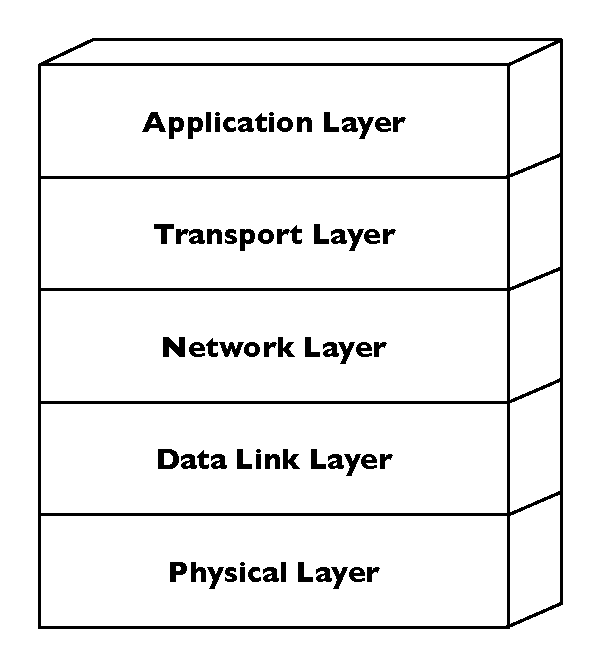
\includegraphics[scale=0.65]{img/ProtStack.eps}
\caption[WSN protocol stack]{WSN protocol stack (reproduced from \cite{SensorSurveyAkyildiz:2002})}
\label{Fig:ProtStack}
\end{figure}

\chapter{Introduction to Wireless Sensor Networks} \label{chap:IntroWSN}
This chapter presents a brief introduction to Wireless Sensor Networks (WSNs)
and its applications. This is followed by a description of the reference
protocol stack used in this work, and the programming abstractions used herein. 
This chapter concludes with examples of typical WSN hardware platforms.

\section{Sensor Nodes} \label{subsec:sensornodes}
WSNs are, as described earlier (see Chapter \ref{chap:Intro}), networks of sensor
nodes, and are typically deployed randomly in a possibly large area where
phenomena are required to be monitored.

As presented in Figure \ref{Fig:SensorNodeArch}, a sensor node consists of
the following elements:
\begin{itemize}
  \item \emph{Sensing unit}, which is comprised of a number of sensors and
  analog-to-digital converters. 
  \item \emph{Transceiver}, which facilitates node-node communication using 
a variety of techniques.
  \item \emph{Processing unit}, that comprises a 
microcontroller/microprocessor that performs processing, and is associated with 
a storage unit.
  \item \emph{Power unit}, which provides the energy required to run the sensor node, and can use chemical 
batteries or power scavenging units such as solar cells.
\end{itemize}

\begin{figure}[h]
\centering
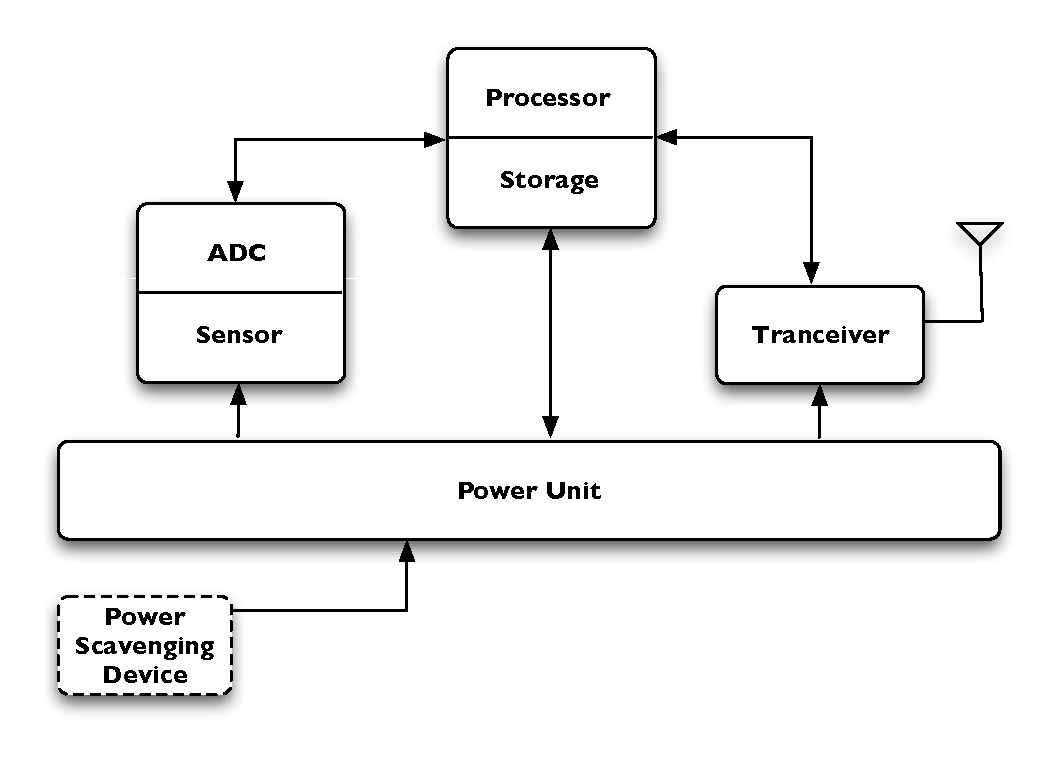
\includegraphics[scale=0.65]{img/SensorNodeArch.eps} 
\caption[Architecture of a sensor node] {Architecture of a sensor node (adapted from \cite{SensorSurveyAkyildiz:2002}).}
\label{Fig:SensorNodeArch}
\end{figure} 

Due to the small size of the devices, sensor nodes have a number of constraints
which affect the WSN built on top of it. These include \cite{yao:qps}:
\begin{itemize}
  \item \emph{Power consumption constraint,} due to the fact that sensor nodes
  have limited energy supply. Therefore, energy conservation is the main concern when
  WSN applications are implemented.
  \item \emph{Computation restriction,} caused by the limited memory
  capacity and processing power available on the sensor node. This places
  serious limitations on the use of data processing algorithms on a sensor node.
  
  \item \emph{Communication constraint,} as a result of the minimal bandwidth available and a
  limited Quality of Service (QoS) provided by the sensor node's hardware. 
\end{itemize}

Additionally, as the deployment of sensor nodes in the WSNs should be
cost-effective, the cost of a single device is a supplementary constraint.

A WSN is self-organising system, given the random nature of the deployment. Its
topology is subject to change because of characteristics of the wireless medium,
and therefore, sensor nodes should be capable of dealing with changes of this kind in order to cope with hostile operating
conditions, the failure-prone nature of sensor nodes and the possibility of
redeployment of additional sensor nodes at any time during operation.

There has been a great deal of interest in WSNs because of several
properties, some of which are listed below: 
\begin{itemize}
  \item Low cost.
  \item Ease of deployment.
  \item Ability to deploy non-invasively in a variety of environments.
  \item High fault tolerance that allows for operation in hostile environments.
  \item High sensing granularity possible.
\end{itemize}

\section{Applications of WSNs}

WSNs have several applications ranging from the military and security domains to
environmental monitoring. This section describes an example of the use of WSNs
to perform fine-grained monitoring of parking bays in a parking lot \cite{benson_carpark}.

Parking lots typically keep track of available spaces using a barrier system
that provides information on vehicles coming in and going out. However, this
approach fails to provide more fine-grained information, such as the
availability of individual parking spaces. WSNs that use RF communication lend
themselves admirably to allowing more fine-grained tracking. 

To implement this, a WSN is deployed in a car park, with a sensor node placed on every
parking bay. When a car is parked on a parking space, it causes a drastic
reduction in the sensor node's communication range, thereby affecting the
pre-existing routing topology. This change in topology can be used to determine
the used and empty parking bays.

\section{WSN Protocol Stack} \label{sec:WSNProtStack}

The WSN protocol stack presented in \cite{SensorSurveyAkyildiz:2002} is an
adaptation of a generic protocol stack \cite{ComputerNetworksTannenbaum:2003}.


\begin{figure}[h]
\centering
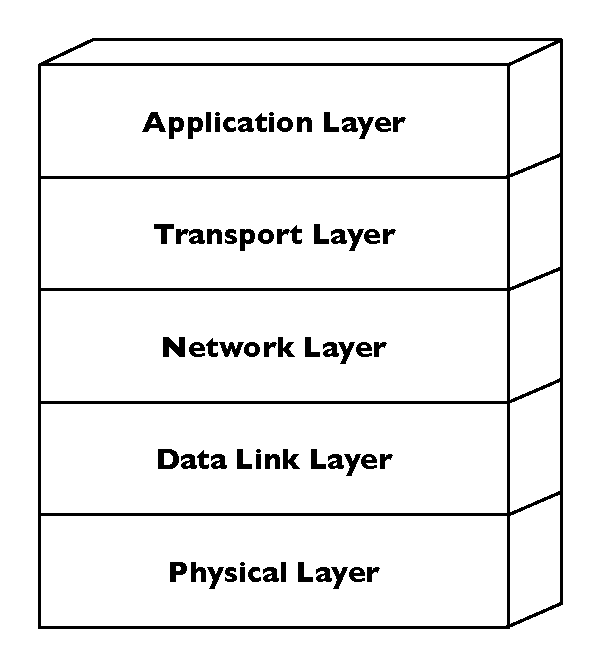
\includegraphics[scale=0.65]{img/ProtStack.eps}
\caption[WSN protocol stack]{WSN protocol stack (reproduced from \cite{SensorSurveyAkyildiz:2002})}
\label{Fig:ProtStack}
\end{figure}

According to \cite{SensorSurveyAkyildiz:2002} the WSN protocol stack consists
of the following layers:

\begin{itemize}
\item \emph{Physical Layer}, which provides the transmission of data over the physical transmission medium.
\item \emph{Data Link Layer}, which deals with power-aware Medium Access Control (MAC) protocols that minimise collisions and transceiver on-time.
\item \emph{Network Layer}, which is primarily responsible for
routing data across the network.
\item \emph{Transport Layer}, which provides reliable delivering of data and
supports error checking mechanisms.
\item \emph{Application Layer}, where the application software resides.
\end{itemize}

The work presented here resides entirely on the application layer of the
protocol stack, and integrates the application layer code with a routing
mechanism that resides in the network
layer.

%\section {Routing in WSNs}

%The existing constraints of the sensor nodes influence the design of routing
%protocols, and these limitations have to be overcome in order to provide
%efficient communication in WSNs \cite{routing:2004}.

%Routing algorithms may be classified on the basis of the organisation of
%the network structure used. Routing algorithms are thus primarily classified
%into being either:
%\begin{itemize}
%\item \emph{Flat}, where every node plays the same role, 
%\item \emph{Hierarchical}, where the network is organised into physically
%defined clusters,
%\item \emph{Location-based}, where positioning information is used to direct
%traffic to a given physical subset of the network.
%\end{itemize}

%Additionally, depending on how the source finds a route to the destination
%routing protocols can be split into three categories \cite{routing:2004}:
%\begin{itemize}
%	\item \emph{Proactive}, when all routes are known before they are used
%	\item \emph{Reactive}, when route is computed on demand 
%	\item \emph{Hybrid}, which uses a combination of the two techniques above.
%\end{itemize}

%The LN routing algorithm that is principal to this work may be considered as an
%exaple of a hybrid routing algorithm, as logical predicates
%are used to direct traffic to a specific \emph{logical} subset of the network.
%A more detailed discussion of the LN mechanism may be found in
%Chapter \ref{chap:background}.

\section {Programming Models for WSNs}

Current WSN programming paradigms are predominantly node-centric, wherein
applications are monolithic and tightly coupled with the protocols and algorithms
used in the lower layers of the protocol stack. 
The main reason for this is the limited resources available on the sensor node, as
was previously discussed in Section \ref{subsec:sensornodes}.

The primary problem with a node-centric approach is that most WSN applications
are developed at an extremely low level of abstraction, which requires the programmer to be knowledgeable in the field of
embedded systems programming. This stunts the growth in the use of WSNs in the
large space of application domains where it may potentially be of use
\cite{mottola_middleware:2008}. 

To increase the ubiquity of WSN
usage, it is essential that protocols and mechanisms underlying WSN
development recede to the background, and the application programmer is
empowered to develop WSN applications at a higher level of abstraction. This
can be achieved using programming models that engineer a shift in focus
towards the system and its results, as opposed to sensor node functionality
itself \cite{mottola_middleware:2008}. 

According to Yu et al \cite{yu_issuesMiddleware:2004}, the use of such
programming models is beneficial for WSN applications because:
\begin{itemize}
\item The semantics of a WSN application can be separated from the details of 
the network communication protocol, OS implementation and hardware.
\item Efficient programming models may facilitate better utilisation of system 
resources.
\item They facilitate the reuse of WSN application code.
\item They provide support for the coordination of multiple WSN applications.
\end{itemize}

\subsection{Taxonomy of WSN Programming Models}

\begin{figure}
\centering
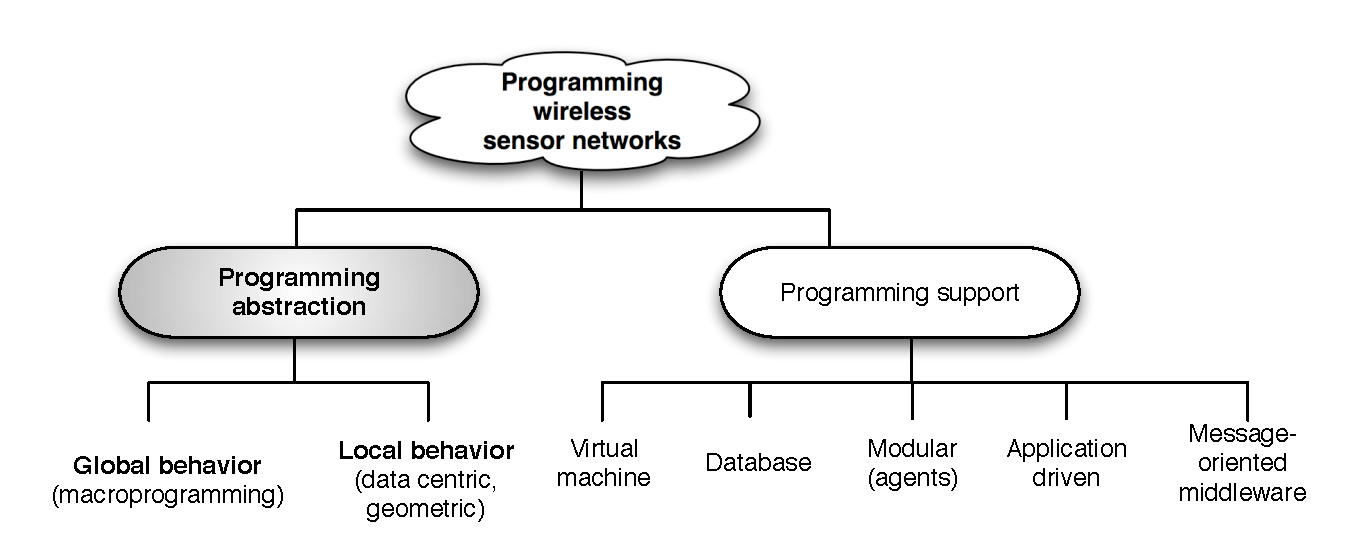
\includegraphics[width=\textwidth]{img/ProgrammingAbstractions.eps} 
\caption[Taxonomy of WSN programming models]{Taxonomy of WSN programming models (reproduced from
\cite{hadim_middleware:2006})}
\label{Fig:ProgrammingModels}
\end{figure}

Existing programming models for WSNs cover different areas and can serve 
several different purposes. They can be classified into two main types, depending on 
the applications they are used for  \cite{hadim_middleware:2006} (see Figure
\ref{Fig:ProgrammingModels}):
\begin{itemize}
\item \emph{Programming support}, wherein services and mechanisms allowing for 
reliable code distribution, safe code execution, etc. are provided. Some
examples of programming models that take this approach include Mate
\cite{Levis_Mate:2002}, Cougar \cite{Bonnet_Cougar:2001}, SOS
\cite{Han_SOS:2005}, and Agilla \cite{Fok_Agilla:2005}.
\item \emph{Programming abstractions}, where models deal with the global view 
of the WSN application as a system, and represent it through the concepts and 
abstractions of sensor nodes and sensor data. Some
examples of programming models that take this approach include Kairos \cite{gummadi_Kairos:2005}, and
EnviroTrack \cite{Abdelzaher_EnviroTrack:2004}.
\end{itemize}

This section further discusses and classifies a subset of WSN programming
models, namely WSN programming abstractions.

Programming abstractions may be distinguished depending on the way WSN nodes
are being programmed, and therefore either be
\emph{global} (also referred to as macroprogramming) or \emph{local} \cite{hadim_middleware:2006}. 

In the former case, the sensor network is programmed as a whole, and gets rid of
the notion of individual nodes \cite{mottola_middleware:2008}. Examples of
macroprogramming solutions include \emph{TinyDB} \cite{madden_TinyDB:2005} and
\emph{Kairos} \cite{gummadi_Kairos:2005}. 

In the latter case, the focus is on identifying relevant sections or
\emph{neighbourhoods} of the network. It is to be noted that these neighbourhoods
need not necessarily be physical. The framework used and developed during the
course of this work belongs to the latter class of programming abstractions.

Programming abstractions may also be classified on the basis of the
nature of the language constructs made available to the WSN programmer
\cite{mottola_middleware:2008}. 

Classification of WSN programming abstractions w.r.t. language constructs is
presented in Figure \ref{Fig:ProgrAbstrClassification}.

\begin{figure}
\centering
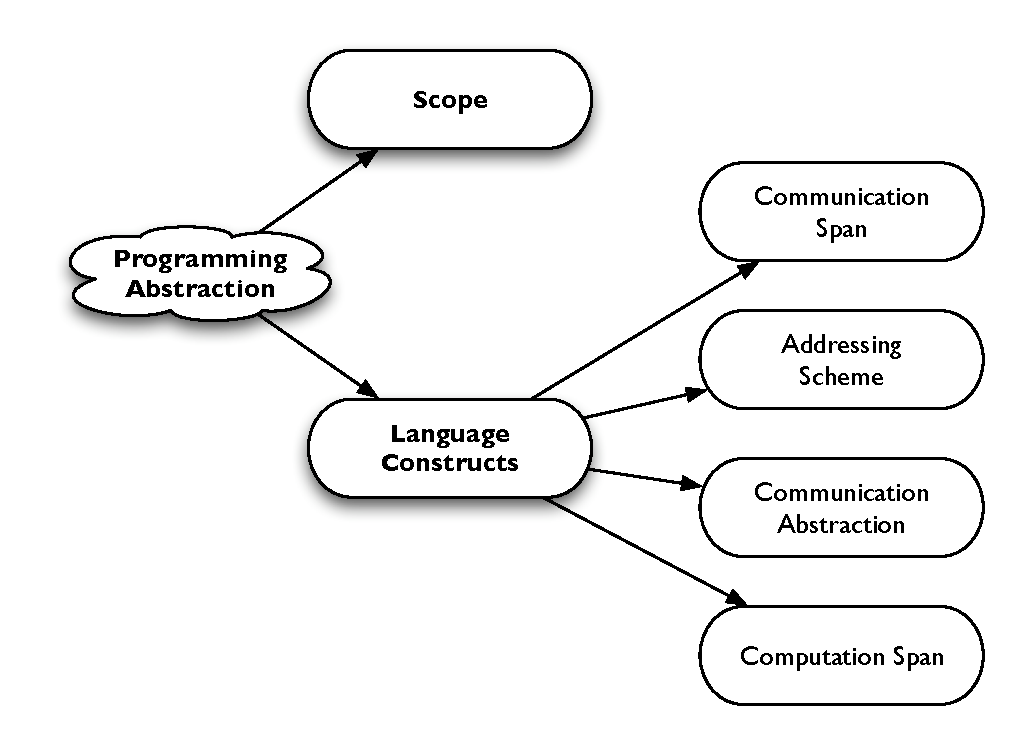
\includegraphics[scale=0.65]{img/ProgAbstr_Classification.eps}
\caption{Classification of Programming Abstractions (adapted from \cite{mottola_middleware:2008})} 
\label{Fig:ProgrAbstrClassification}
\end{figure} 

The rest of this section discusses each of these bases for classification in
detail, and is based on the work described in \cite{mottola_middleware:2008}
unless explicitly mentioned otherwise.

\subsubsection{Communication Span}

The \emph{Communication span} enabled by a WSN programming interface is defined
as the set of nodes that communicate with one another in order to accomplish a
task. The communication span provided by a given abstraction can be
\cite{mottola_middleware:2008}:
\begin{itemize}
  \item \emph{Physical neighbourhood}
  \item \emph{Multi-hop group}
  \item \emph{System-wide}
\end{itemize}

Abstractions that use \emph{physical neighbourhood} approach provide
  the programmer with constructs to allow nodes to exchange data with others
  within direct communication range. Examples of communication in physical
  neighbourhood include nesC \cite{nesc:2003} and Active Messages \cite{activemessagesEicken:2001}.
  
Abstractions using the \emph{multi-hop group} approach allow the
  programmer to exchange data among subsets of nodes in the WSN using
  multi-hop communication. These sets may either be
  \emph{connected}, wherein there always exists a path between any two nodes in
  the set, or \emph{non-connected/disconnected}, where ``no assumptions on the geographical location of nodes 
belonging to the group'' \cite{mottola_middleware:2008} can be made.  
  The EnviroSuite Framework \cite{envirosuite:2006} represents an example of
  connected multi-hop communication, as do Logical Neighborhoods
  \cite{mottola_LN:2006} - an example of non-connected multi-hop
  communication.

\emph{System-wide} abstractions let the
  programmer use constructs that allow data exchange between any two nodes
  in the WSN. This may be seen as an extreme manifestation of the
  \emph{multi-hop group} approach mentioned above. An example of system-wide
  communication is the TinyDB \cite{madden_TinyDB:2005} project.
  
\subsubsection{Addressing Scheme}

The \emph{addressing scheme} specifies the mechanism by which nodes are
identified. Typically, there are two kinds of addressing schemes used
\cite{mottola_middleware:2008}:

\begin{itemize}
  \item \emph{Physical addressing}
  \item \emph{Logical addressing}
\end{itemize}

In \emph{physical addressing} schemes nodes are identified using unique 
  identifiers. The same address always identifies the same node (or nodes, if
  duplicate  identifiers exist) at any time during the execution of the
  application. The paradigmatic example of a physical addressing scheme is
  Active Messages communication \cite{activemessagesEicken:2001}.

When a \emph{logical addressing} mechanism is used, nodes are identified on the
basis of application-level properties specified by the application
programmer. Therefore, the same address, i.e., the set of
application-level predicates, can identify different sets of nodes at different
times. An example of logical addressing is Logical Neighborhood communication
\cite{mottola_LN:2006}.

\subsubsection{Communication Abstraction}

This classification basis defines the degree to which details of communication
in a WSN are hidden from the application programmer's view. Programming
interfaces may provide either \cite{mottola_middleware:2008}:
\begin{itemize}
  \item \emph{Explicit communication} primitives where the
  programmer working in the application layer has to handle communication
  aspects such as buffering and parsing. 
  \item \emph{Implicit communication}, where the programmer is unaware of the
  details of the communication process, and communicates using
  high-level constructs.
\end{itemize}

Active Messages \cite{activemessagesEicken:2001} are an example of
an explicit communication approach. In contrast, the Active Regions programming
framework \cite{activeregions:2004} belongs to the latter category.

\subsubsection{Computation Span}

The \emph{Computation span} enabled by a WSN programming interface is defined
as the set of nodes that can be affected by the execution of a single
instruction. The
computation span provided by a given abstraction can be
\cite{mottola_middleware:2008}:

\begin{itemize}
  \item \emph{Node}, when the effect of any instruction is restricted to a
  single node.
  \item \emph{Group}, where the programmer is provided with constructs that
  could affect a subset of nodes. 
  \item \emph{Global} present an extreme case of previous type, a single
  instruction can impact every node in the WSN.
\end{itemize}

An example of node computation is the ATaG framework \cite{atag:2005}, while the
Regiment system \cite{regiment:2007} implements a group communication approach.
TinyDB \cite{madden_TinyDB:2005} represents an example of global computation
span.

\subsection{Programming Models on the WSN Protocol Stack}

\begin{figure}
\centering
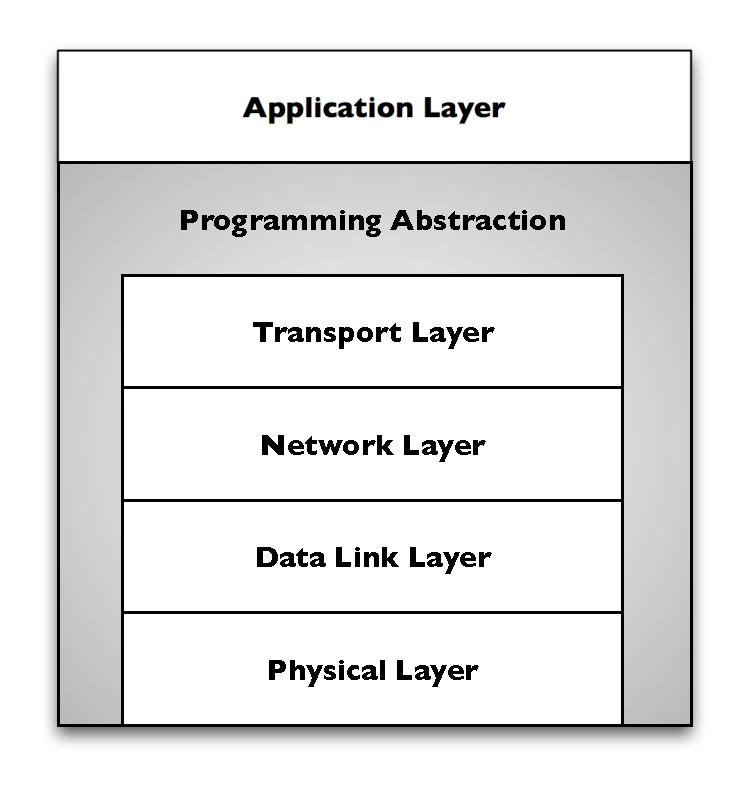
\includegraphics[scale=0.61]{img/ProtStack_ProgAbstr.eps}
\caption[Programming models on the WSN protocol stack]{Programming models on the WSN protocol
stack (adapted from \cite{mottola_middleware:2008})}
\label{Fig:ProtStack_ProgAbstr}
\end{figure}

WSN programming models are typically placed between the application layer and
the
transport layer in the protocol stack shown in Section \ref{sec:WSNProtStack}. As it can be seen from
Figure \ref{Fig:ProtStack_ProgAbstr},
fine-grained details are hidden from the application programmer's view. These
include:

\begin{itemize}
  \item Higher-layer services such as routing, localisation, and data storage
  mechanisms (and optimisations).
  \item Lower-layers such as the MAC protocol used, and the physical means of
  communication such as RF communication.
\end{itemize}

\section{Hardware Platforms}

There exist several hardware platforms for WSN development, a few of which are
described here.

\subsection{Sun SPOTs}

Sun SPOTs \cite{simon_squawk:2006,sun_developer:2008} are sensor devices built
upon the IEEE 802.15.4 standard by Sun
Microsystems, and are programmed using a subset of the Java managed-runtime
programming
language. Programs written for Sun SPOTs are run on the Squawk Java Virtual
Machine (JVM). Sun SPOTs were the hardware platform used for the evaluation of
this work, and are described in greater detail in Section \ref{sec:sunspots}.

\subsection{Tmote Sky}

The Tmote sky is an IEEE 802.15.4 compliant sensor device
\cite{tmote_sky_brochure:xxxx} developed by moteiv
(now Sentilla). It uses an MSP430 microcontroller, provides 10 kB of RAM,
48 kB of program space, and 1024 kB of external Flash memory, and can transfer
data at the rate of 250 kBps in the 2.4 GHz Industrial-Scientific-Medical (ISM)
band. These devices run the TinyOS Operating System (OS) \cite{levis_tinyos:2005}, and are programmed
using the nesC programming language \cite{gay_nesc}.

\subsubsection{The Sentilla Mini}

Moteiv has been acquired by Sentilla, and have released a Java-compliant 
MSP430-based sensor
device with a smaller form factor than that of the Tmote sky, called the
Sentilla mini\footnote{http://www.sentilla.com/hardware.html}.

\section{Summary}
This chapter presented an introduction to WSNs and discussed in detail the 
sensor nodes that constitute them. This was followed by a description of WSN
applications, and the
WSN protocol stack. The chapter then concluded with a description of WSN
programming models and hardware platforms.
\chapter{Background} \label{chap:background}

%% REWRITE!??

This chapter presents a brief discussion of the concepts and algorithms
that were used during the course of this work. 

This chapter begins with presentation of abstract data types and
discusses its applicability for WSNs. The chapter further presents distributed
abstract data types (DADTs) and concepts underlying them \cite{migliavacca_DADT:2006}.

This is followed by a brief presentation of the Logical Neighborhoods (LN) \cite{mottola_LNScoping:2006}, a mechanism that
enables routing and scoping in WSNs.  

%This
%chapter begins with an introduction to programming abstractions and continues
%with a discussion on their applications in WSN programming.

%This chapter further presents the concepts underlying Distributed Abstract Data
%Types (DADTs) \cite{migliavacca_DADT:2006}. This is followed by a presentation
%of the Logical Neighborhoods (LN) \cite{mottola_LNScoping:2006}, a mechanism
%that enables routing and scoping in WSNs. 

%The chapter then concludes with a
%description of the hardware platform - Sun Small Programable Object Technology
%(SPOT) \cite{simon_squawk:2006} - used to experimentally validate the
%implemented prototype in a real-world environment.

\section{Abstract Data Types}

An Abstract Data Type (ADT) is the depiction of a model that
presents an abstract view to the problem at hand. This model of a problem
typically defines the affected data and the identified operations associated with
those.

The set of the data values and associated operations, independent of any
specific implementation, is called an ADT \cite{NIST_website}. From the
application developer's point of view, the use of ADTs allows for the separation of
interfaces from specific implementations.

One may consider a \emph{stack} as a simple example of an ADT
\cite{guttag_ADTs:1977}. It can be represented through the stacked data, and a set of defined
operations that include \emph{push(data)}, \emph{pop()}, and \emph{top()}. It is intuitively clear that
several different implementations of an ADT may be defined using the proposed specification.


%\subsection{ADTs in WSNs} \label{subsubsec:ADTsinWSN}

The concept of ADTs has been successfully used in several different areas of
science. This idea clearly has found its applicability in WSNs, due to
possibility to separate interfaces provided by sensor nodes and their particular
implementations. 

%The rest of this section focuses on the application and extension of the concept of ADTs for use in WSNs.

A top-down aproach can be used to overview an abstraction of WSN and its parts.
Any WSN as described earlier, usually consists of a number of sensor nodes, where each
sensor node may include several sensors used to measure specific phenomenon.

\begin{figure}[h]
\centering
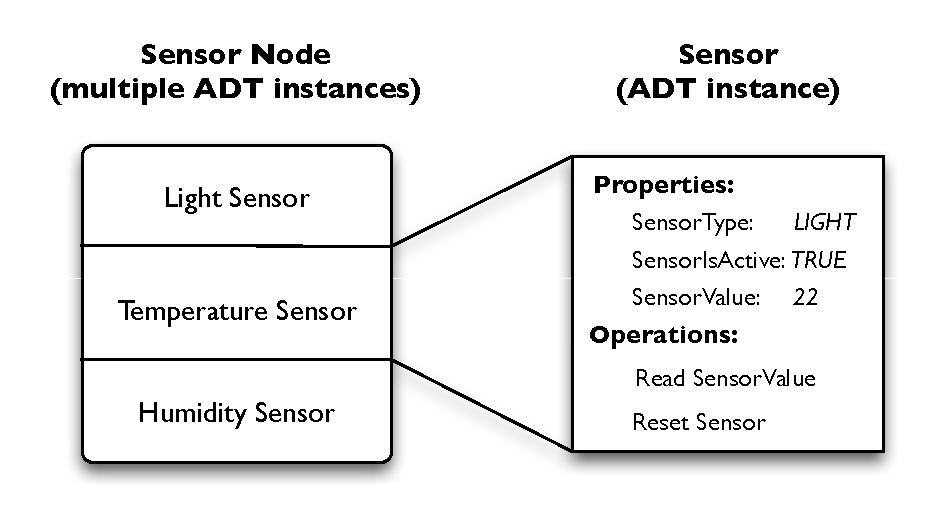
\includegraphics[scale=0.71]{img/ADTsMultipleInstances.eps}
\caption[Abstraction of sensor node through multiple ADTs]{Abstraction of sensor node through multiple ADTs}
\label{Fig:MultipleADTs}
\end{figure} 
  
Referring to the example in Figure \ref{Fig:MultipleADTs}, the ADT instance
\emph{Sensor} can be used to abstract different types of sensors that may be
present on a sensor node. It specifies that a \emph{Sensor} provides the list of
common properties and operations. By declaration of multiple such ADT instances,
the nature of the wireless sensor node can be abstracted, as can be seen in the
\emph{Sensor Node} entity shown in Figure \ref{Fig:MultipleADTs}. This then
allows the ADT instances to be used by the application developer at a later
point\footnote{Further details of ADT specification and instantiation are
provided in Section \ref{subsec:ADTSpecInst}}.

\section {Distributed Abstract Data Types} \label{sec:DADT}

Distributed Abstract Data Types present a new programming language construct
used to support distributed and context-aware applications. The concept of DADTs was
introduced in \cite{migliavacca_DADT:2006}, and based on the notion of ADTs,
which are divided into two classes - data and space ADTs. 
The rest of this section presents the concepts and provides the reader with the
relevant background and examples\footnote{The examples provided are adapted from \cite{migliavacca_DADT:2006}}.

\subsection{Data and Space ADTs} \label{subsubsec:DataAndSpaceADTs}

It is important to distinguish between data required by an application, and
the location, or space, where the providers of data reside. ADTs in WSNs can
provide not only the data from the sensor node, but also express a notion
of the ``computational environment'' hosting the data ADT.

Thus, ADTs be of two types:

\begin{itemize}
  \item \emph{Data ADTs}
  \item \emph{Space ADTs} 
\end{itemize}

\emph{Data ADTs} are ``conventional'' ADTs which encode application logic, such
as, for instance, allowing access to sensor data.

\emph{Space ADTs}, also known as \emph{sites}, are ADTs that provide an
abstraction of the computational environment (in the case of a WSN, a sensor
node) that ``hosts the data ADT'' \cite{migliavacca_DADT:2006}. The space ADT may
use different notions of space, such as physical location or network topology,
depending on application requirements as determined by the programmer.

\subsection{DADTs as an extension of ADTs} \label{subsec:DADTsConcepts}
Distributed ADTs (DADTs) are an extension of ADTs that make the state of multiple ADTs in a
distributed system collectively available.
\cite{migliavacca_DADT:2006}. 

\begin{figure}[h]
\centering
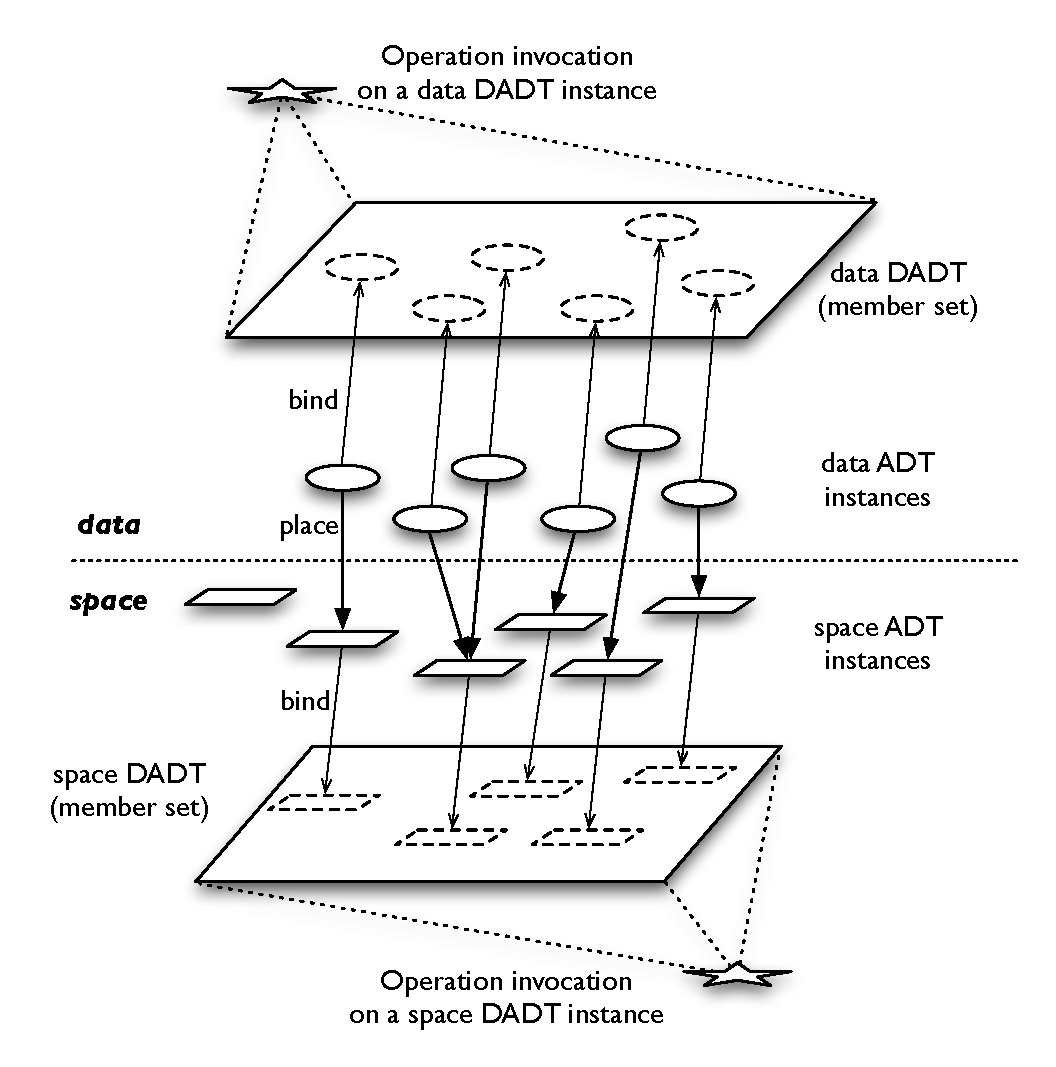
\includegraphics[scale=0.65]{img/DADTs.eps} 
\caption[Data and space in the DADT model]{Data and space in the DADT model (reproduced from 
\cite{migliavacca_DADT:2006})}
\label{Fig:DADTs}
\end{figure}

Similar to ADTs, DADTs 
provide specifications for distributed data, distributed operators, and 
constraints. The notion of space is extended to DADTs, and therefore DADTs can
either be (as it is shown in the Figure \ref{Fig:DADTs}):

\begin{itemize}
  \item \emph{Data DADT} that provide distributed access to a collection of data
  ADTs.
  \item \emph{Space DADT} that allows distributed access to a collection of
  space ADTs. 
\end{itemize}

The set of ADTs that are available for collective access using a DADT is called the \emph{member set} of
the DADT.

\subsubsection{DADT Operators and Actions} \label{subsubsec:OperatorsAndActions}

Operators are used in DADTs to declare distributed references to
the ADTs in the DADT member set. This reference conceals identities of individual ADT
instances from the application programmer. 

DADT operators may belong to one of the following types:

\begin{itemize}
  \item \emph{Selection Operators} that allow the performance of
  distributed operations on a subset of the instances in the member set.
  Examples of such operators could be \emph{all}, or \emph{any} selection
  operator, because they allow to declare a subset of the instances.

  \item \emph{Conditional Operators} that provide support for global
  conditions to be applied on the member set prior to the execution of the DADT
  operation. One of the examples of conditional operator is operator
  \emph{in}, that allows to check if one set of instances contains in another
  one.

  \item \emph{Iteration Operators} that allow iterating over the
  ADT instances in the set, and thus permit access to individual ADT instances.
  Examples of such operators are \emph{next}, \emph{previous}, \emph{last},
  \emph{first}, as they allow to address and iterate over the members of the
  set.
\end{itemize}

The DADT operators described above allow different way to access ADT
instance and execute one of the ADT operations defined in the
ADT specification.

Distributed appliation developer may require to implement more complicated
application logic, though it may happen that even available ADT operations
are not sufficient. In this case the special DADT construct, called DADT
action, can be used \cite{migliavacca_DADT:2006}. 

DADT actions are specified by the DADT type, but are executed similarly to ADT
 operation on remote ADT instances.

\subsubsection{Views} \label{subsubsec:views}

\emph{DADT Views} permit the definition of the scope of distributed operations
that the application requires to perform. This approach is particularly useful
when a distributed operation has to be executed only on a subset of the
member set of ADT instances. The concept of DADT Views is presented in Figure
\ref{Fig:DADT_Views}.

\begin{figure}[h]
\centering
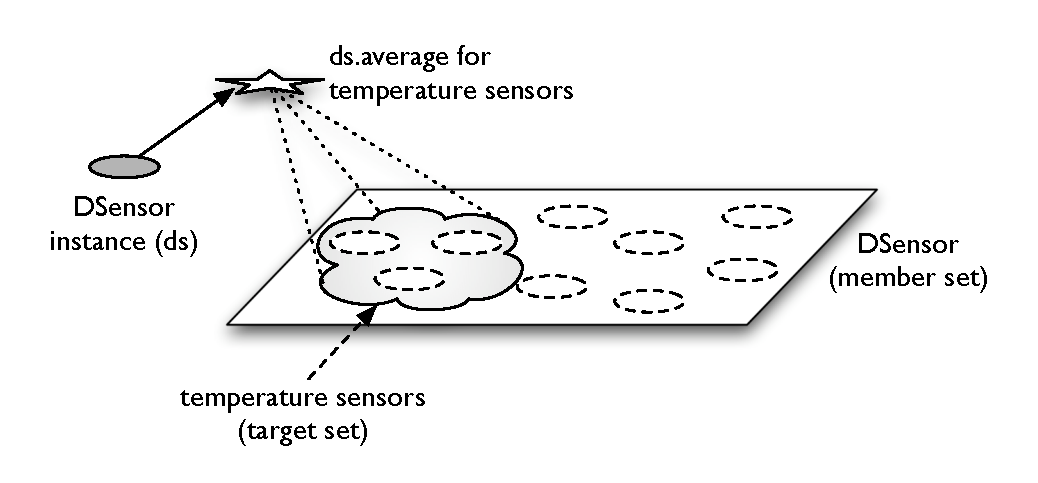
\includegraphics[scale=0.75]{img/DADT_Views.eps} 
\caption[DADT Views]{DADT views (reproduced from \cite{migliavacca_DADT:2006})}
\label{Fig:DADT_Views}
\end{figure}

The member set may be partitioned into DADT Views by using properties. A
\emph{Property} is a DADT characteristic that is defined in terms of an ADT's
data and operations, and is evaluated locally on the ADT instance
\cite{migliavacca_DADT:2006}. DADT View may either be:
\begin{itemize}
  \item \emph{Data View},
  \item \emph{Space View}.
\end{itemize}

Application developer should decide what could be the best
way to access the WSN. A Data DADT instance can be used to
operate on the distributed data and limit the scope using predicates over
DADT properties representing data, space, or both,
depending on the needs of the application. Similarly, any kind of view to
access the distributed representation of Space can be applied.

This section has presented concepts underlying the DADTs. A brief description
of the DADT prototype \cite{migliavacca_DADT:2006} will be presented further in
Section \ref{sec:DADTPrototype}.

\subsection {The DADT Prototype} \label{sec:DADTPrototype}

The DADT prototype implemented by Migliavacca et al \cite{migliavacca_DADT:2006}
was written in Java, and presents the design of a DADT specification language
that extends Java.

This section provides the reader with
further details on the concepts central to DADTs\footnote{All the DADT concepts presented below
are described using the DADT specification language.}, a description of the
existing DADT prototype \cite{migliavacca_DADT:2006}, and a discussion on its limitations.

\subsection{ADTs Specification and Instantiation} \label{subsec:ADTSpecInst}

As was mentioned in Section \ref{subsubsec:ADTsinWSN}, each sensor node
in a WSN can be abstracted using multiple ADT instances (see
Figure \ref{Fig:MultipleADTs}), and therefore conceal the details of sensor
node abstraction from the application developer. The code snippets below are
provided to illustrate these concepts.

The specification of a described ADT may be defined as a Java
class, as shown in Listing \ref{listing:ADTSpec}

\begin{lstlisting}[frame=trbl, basewidth={0.55em, 0.6em}, captionpos=b,
basicstyle=\ttfamily\footnotesize, breaklines, caption = Sensor ADT instances, label =
listing:ADTSpec]
class Sensor {
  //data properties of the sensor 
    int sensorType;
    double sensorReading;
    boolean active; 
  //operations that can be performed on the sensor  
    public double read(){ //read the sensor value.
    ...
    } 
    public void reset(){ //reset the sensor
    ...
    }    
\end{lstlisting}
 
This specification declares that a Sensor ADT instance should provide the following properties:
\begin{itemize}
\item an integer value to define the sensor type,
\item a double value that holds the sensor data, 
\item a boolean value that stores information about sensor's state of activity.
\end{itemize}
as well as operations that allow to \emph{Read} sensor data and \emph{Reset}
the sensor.

It is possible to define multiple such instances of this specification. For
example, the ADT instances for a given sensor node that has two kinds of sensors
- (a) a temperature sensor, and (b) a light sensor - may be defined using the ADT
specification described above, as shown in Listing \ref{listing:ADTInstances}. 
\begin{lstlisting}[frame=trbl, basewidth={0.55em, 0.6em}, captionpos=b,
basicstyle=\ttfamily\footnotesize, breaklines, caption = Sensor ADT instances, label =
listing:ADTInstances]
  // Temperature sensor ADT instance
    Sensor temperatureSensor = new Sensor(TEMPERATURE);
  // Light sensor ADT instance  
    Sensor lightSensor = new Sensor(LIGHT);
\end{lstlisting}

\subsection{DADT Specification and Instantiation} \label{subsubsec:dadtspecandinst}

The concept of DADTs was first introduced in Section \ref{sec:DADT}, and will
be extended in this chapter with examples of DADT specification and
instantiation.

DADT specifications can be best understood by carrying forward the example
described in Section \ref{subsec:ADTSpecInst}. To allow for collective access
to multiple ADT instances of the type specified in Listing
\ref{listing:ADTSpec}, a DADT \emph{DSensor} may be defined as shown in Listing
\ref{listing:DADTSpec}.   
 
\begin{lstlisting}[frame=trbl, basewidth={0.55em, 0.6em}, captionpos=b, 
basicstyle=\ttfamily\footnotesize, breaklines, caption = Data DADT 
specification (reproduced from \cite{migliavacca_DADT:2006}), label = listing:DADTSpec]
class DSensor distributes Sensor{	
  //properties:
    property isSensorType(int type);
    property isActive();

  // distributed operations:
    distributed double average()	
    distributed void resetAll();
}
\end{lstlisting} 
 
This DADT specification allows two simple distributed operations to be performed
on multiple data ADTs of type \emph{Sensor}:  
\begin{itemize}
\item \emph{resetAll()} 
\item \emph{average()} 
\end{itemize}

The \emph{resetAll()} operation is used to reset every sensor in the DADT member
set, or subset of ADT instances defined by a DADT View (see Section
\ref{subsubsec:views}).

The \emph{average()} operation allows for the calculation of the average of the readings of every
sensor in the member set, or the subset of it defined by the DADT view.

Additionally, the DADT specification  shown in Listing \ref{listing:DADTSpec}
declares two DADT Properties described later.

Listing \ref{listing:DADTInstance} shows how DADT specifications can be
instantiated as an object of a Java class, and be used to perform defined
distributed operations.

\begin{lstlisting}[frame=trbl, basewidth={0.55em, 0.6em}, captionpos=b, 
basicstyle=\ttfamily\footnotesize, breaklines, caption = DADT Instantiation 
(reproduced from \cite{migliavacca_DADT:2006}), label = listing:DADTInstance ]
  DSensor ds = new DSensor();
  ds.resetAll();
\end{lstlisting}

\subsection{Binding ADTs to DADTs}

As mentioned earlier in Section \ref{subsec:DADTsConcepts}, a DADT member set
consists of the set of ADTs that are available for collective
access, which, in the given example, is the collection of ADTs of type \emph{Sensor}.

An ADT instance is made part of the member set by binding it to the DADT type.
This can be done using a dedicated programming construct \emph{bind} as shown in
Listing \ref{listing:binding}, where the Sensor ADT defined in Listing
\ref{listing:ADTSpec} is bound to the DADT type \emph{DSensor} defined in Listing \ref{listing:DADTSpec}.
 
\begin{lstlisting}[frame=trbl, basewidth={0.55em, 0.6em}, captionpos=b, 
basicstyle=\ttfamily\footnotesize, breaklines, caption = Binding ADT instances to a DADT instance, label = listing:binding]
  bind(new Sensor(TEMPERATURE), "DSensor");
  bind(new Sensor(LIGHT), "DSensor");
  ...
\end{lstlisting} 

Binding of ADT instances takes place on the sensor device that holds sensors,
as those are abstracted into specific ADTs.

\subsection{Implementing DADT Operators and Actions}
\label{subsubsec:OperatorsAndActionsImpl}

The concepts of DADT Operators and Actions were already introduced in the
previous chapter (see Section \ref{subsubsec:OperatorsAndActions}). This
section describes the implementation of Operators and Actions in the DADT
prototype \cite{migliavacca_DADT:2006}.

\subsubsection{DADT Operators}
Listing \ref{listing:DADTOperator} extends the example first introduced in
Listing \ref{listing:DADTSpec}, and presents the use of the DADT selection
operator \emph{all}.

\begin{lstlisting}[frame=trbl, basewidth={0.55em, 0.6em}, captionpos=b, 
basicstyle=\ttfamily\footnotesize, breaklines, caption = Use of DADT Selection Operator, label = listing:DADTOperator]  
class DSensor distributes Sensor{
  ...
  distributed void resetAll(){
    (all in targetset).reset();
  }
}
\end{lstlisting}

The distributed operation \emph{resetAll} uses the selection operator 
\emph{all} in order to gain access to all ADT instances in the DADT
target set, and subsequently invokes the \emph{reset} operation on the ADT
instance. The \emph{reset} operation was declared in the ADT specification
shown in Listing \ref{listing:ADTSpec}.

\subsubsection{DADT Actions}
However, if the application developers finds the set of available ADT operations limited, he/she has the option of using DADT actions that are defined in the DADT type and executed locally on the ADT instance.

DADT actions do not necessarily consist only of single ADT operations, but can
also implement more complicated logic. For instance, a
\emph{reliableRead} action may be implemented that is capable of handling sensor read failures by means of performing multiple read attempts, failing which
a sensor node reset is performed (See Listing \ref{listing:DADTAction}).
 
\begin{lstlisting}[frame=trbl, basewidth={0.55em, 0.6em}, captionpos=b, 
basicstyle=\ttfamily\footnotesize, breaklines, caption = Use of DADT Action (reproduced from \cite{migliavacca_DADT:2006}), label = listing:DADTAction]  
class DSensor distributes Sensor {
  distributed double average(){
  ...  
  action double reliableRead(){
    double reading;
      int tries = 3;
      while (tries > 0){
        reading = local.read();  // use of ADT operation
        if (reading == ERROR) --tries;
        else break; 
      }
      if (reading == ERROR) {
        local.reset();
        reading = local.read();
      }
    }

    double[] sensorReadings = (all in targetset).reliableRead();
    ...
    // evaluation of the average value based on received readings	
    ...
    }
}
\end{lstlisting}

\subsection{DADT Views} \label{subsubsec:viewsImpl}

DADT Views are an effective tool for the application developer to
define the scope of a distributed operation. As was described in the Section
\ref{subsubsec:views}, DADT Views are created using DADT properties.

To continue to use the example running throughout this section, if the application programmer wishes to refer to a subset of temperature sensors from among the member set of ADT instances bound to the DADT type \emph{DSensor}, a data view \emph{TempSensors}, 
as shown in Listing \ref{listing:DADTview}, can be declared.
  
\begin{lstlisting}[frame=trbl, basewidth={0.55em, 0.6em}, captionpos=b, 
basicstyle=\ttfamily\footnotesize, breaklines, caption = Definition of DADT Data View, label = listing:DADTview ]  
dataview TempSensors on DSensor as isSensorType(TEMPERATURE) && isActive(); 
\end{lstlisting}

The DADT name \emph{DSensor} in this case refers to its member set, and 
the data view \emph{TempSensors} is defined as a subset of this member set and
consists only of sensor nodes with temperature sensors for which the evaluation of
both DADT properties (See Listing \ref{listing:DADTProperty}) \emph{isActive}
and \emph{isSensorType} return \emph{true}. 

\begin{lstlisting}[frame=trbl, basewidth={0.55em, 0.6em}, captionpos=b, 
basicstyle=\ttfamily\footnotesize, breaklines, caption = Definition of DADT Properties, label = listing:DADTProperty ]  
class DSensor distributes Sensor {
  property isSensorType(){
	 return (local.type == type);
  }
  property isActive() {
	return local.isActive();
  }
  ...
}

\end{lstlisting}

This section has described the DADT prototype presented in
\cite{migliavacca_DADT:2006}, which was modified and extended to use in WSNs. 
Chapter \ref{chap:design} provides further details about limitations of the
given prototype and presents the DADT/LN prototype. 

\section {Logical Neighborhoods} \label{LNDescription}

Typically, communication between WSN nodes is based on routing 
information between nodes by exploiting the communication radius of each node.
The notion of a node's physical neighbourhood - the set of nodes in the
network that fall within the communication range of a given node - is central to a mechanism of this nature.

However, in heterogenous WSN applications, the developer might require to
communicate with a specific subset of the network that is defined logically and
not physically. As an example of this, consider the following case. An
application that provides security in a high-risk environment by monitoring 
motion might require - in the event of a security alarm - all sensors at the
entrances to the guarded area to report about detected motion.
The sensors at the entrance form a logical neighbourhood in this case. However,
as the entrances may be widely separated, it is not for granted that these nodes
constitute part of a single physical neighbourhood.

The use of current WSN programming techniques to enable a mechanism of this
nature entails additional programming effort, because the developer has to deal
not only with the application logic, but also with the underlying problems of
transmitting messages to a specific logical neighbouhood while using lower layer
constructs that have no notion of this. This leads to increased code complexity
\cite{mottola_LN:2006}.

\begin{figure} 
\centering
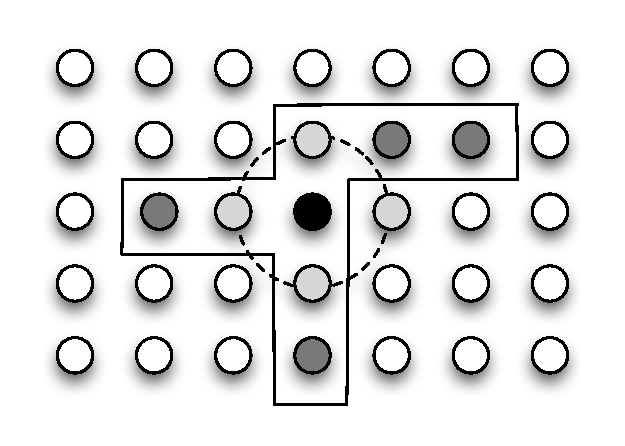
\includegraphics[scale=0.71]{img/LN_physical_vs_logical.eps} 
\caption[Difference between physical and logical neighborhoods]{Representation 
of logical and physical neighborhood of a given node. (reproduced from
\cite{mottola_LN:2006})}
\label{Fig:LN_physical_vs_logical}
\end{figure} 

Mottola and Picco \cite{mottola_LN:2006} suggest the addressing of the
aforementioned issues using \emph{Logical Neighbourhoods (LNs)}, an
abstraction that replaces the node's physical neighbourhood with a logical notion of
proximity. 

Figure \ref{Fig:LN_physical_vs_logical} provides comparison between
physical and logical neighbourhoods. The black node represents the node
that defines the sensor node with its neighbourhoods. The light grey nodes
connected by the dashed circle represent the physical neighborhood, whereas the
dark grey ones with the solid polygon represent (one of the nodes in) the
node's logical neighborhood.


Using this
abstraction, programmers can communicate with members of a LN using a simple message passing API,
thereby allowing for logical broadcasts. The implementation of this API is
supported by means of a novel routing mechanism devised specifically to support
LN communication. 

\subsection{The LN Abstraction}

LNs can be specified using a declarative language such as SPIDEY
\cite{mottola_LN:2006, mottola_LNScoping:2006}, and
involves the definition and instantiation of the \emph{node} and the
\emph{neighbourhood}. 

Nodes are a logical representation of the subset of a sensor node's state and
characteristics, and are used for the specification of an LN. Nodes are defined
in a node template and are subsequently instantiated, as shown in Listing \ref{listing:LN1}
   
A neighbourhood can be defined by applying predicates on the attributes defined
in the node template. The neighbourhood is defined using a neighbourhood
template, and subsequently instantiated.
   
\begin{lstlisting}[frame=trbl, basewidth={0.55em, 0.6em}, captionpos=b, 
basicstyle=\ttfamily\footnotesize, breaklines, caption = Node Definition and Instantiation, label = listing:LN1]  
node template Sensor
  static Function
  static Type
  dynamic BatteryPower
  dynamic Reading

create node ts from Sensor
  Function as "Sensor"
  Type as "Temperature"
  Reading as getTempReading()
  BatteryPower as getBatteryPower()
\end{lstlisting}


Listing \ref{listing:LN2} shows the definition and
instantiation of a
neighbourhood - based on the node template defined in Listing \ref{listing:LN1}
- which selects all temperature sensors where the reading exceeds a threshold.
 
\begin{lstlisting}[frame=trbl, basewidth={0.55em, 0.6em}, captionpos=b, 
basicstyle=\ttfamily\footnotesize, breaklines, caption = Neighbourhood Definition and Instantiation, label = listing:LN2]  
neighbourhood template HighTempSensors(threshold)
  with Function = "Sensor" 
      and Type  = "Temperature" 
      and Reading > Threshold

create neighbourhood HigherTemperatureSensors
  from HighTempSensors(threshold:45)
\end{lstlisting}

LN communication is enabled using a simple API that overrides the
traditionally used broadcast facility and makes it dependent on the (logical)
neighbourhood the message is addressed to \cite{mottola_LN:2006}. The underlying routing mechanism is presented in further
details in \cite{mottola_LN:2006, mottola_LNScoping:2006}.

\section{Summary}

This chapter presented an overview of the concepts, technologies, and hardware
underlying the work presented in this thesis. After underlining the need for the
use of programming models to increase the ubiquity of WSN use, this chapter
introduced a taxonomy of programming abstractions and placed the Distributed
Abstract Data Types programming abstraction used in this work within the
framework of the taxonomy. This was followed by a detailed discussion on Abstract
and Distributed Abstract Data Types used in the application layer of the
prototype produced during the course of this work, and the Logical Neighbourhood
routing mechanism used in the network and data link layers of the prototype. 


  
\chapter{Tools} \label{chap:tools}

\section{simulator - rename}

\section {Sun SPOTs} \label{sec:sunspots}

Sensor nodes, as mentioned in Section \ref{subsec:sensornodes}, are
characterised by limited resources, including memory. 

In order to overcome memory limitations, wireless sensor network applications
have traditionally been coded in non-managed languages like C and assembly
language \cite{simon_squawk:2006}.
 
Managed runtime languages like Java were not used for sensor network programming
because of the combination of the static memory footprint of the Java Virtual
Machine (JVM) and the dynamic memory footprint of the WSN application code.
 
On the other hand, it is widely accepted that development times are greatly reduced
upon the use of managed runtime languages such as Java
\cite{simon_squawk:2006}. Therefore, currently prevalent WSN programming practice
trades developer efficiency for memory efficiency. 

However, Simon et al \cite{simon_squawk:2006} state the benefits resulted from
using a managed runtime language for WSN programming as follows:

\begin{itemize}
  \item Simplification of the process of WSN programming, that would cause an
  increase in developer adoption rates and productivity.
  \item Opportunity to use standard development and debugging tools.
\end{itemize}

The use of the Java programming language in SunSPOTs makes it particularly
suitable as a platform for the DADT applications presented. This is because the
DADT programming abstraction is designed to reduce programmer workload, and the
use of a managed runtime language such as Java has been shown to further
improve developer efficiency.
 
\subsection{The Sun SPOT hardware platform }
Sun Microsystems has, on the basis of the arguments discussed in the previous
section, proposed and built a sensor device
called the Sun Small Programmable Object Technology (Sun SPOT) that uses a
on-board JVM to allow for WSN programming using Java.

The Sun SPOT (see Figure \ref{Fig:SunSpot}) uses an ARM-9 processor, has 512 KB of RAM
and 4 MB of flash memory, uses a 2.4GHz radio with an integrated antenna on the board. The radio
is a TI CC2420 and is IEEE 802.15.4 compliant.

\begin{figure} 
\centering
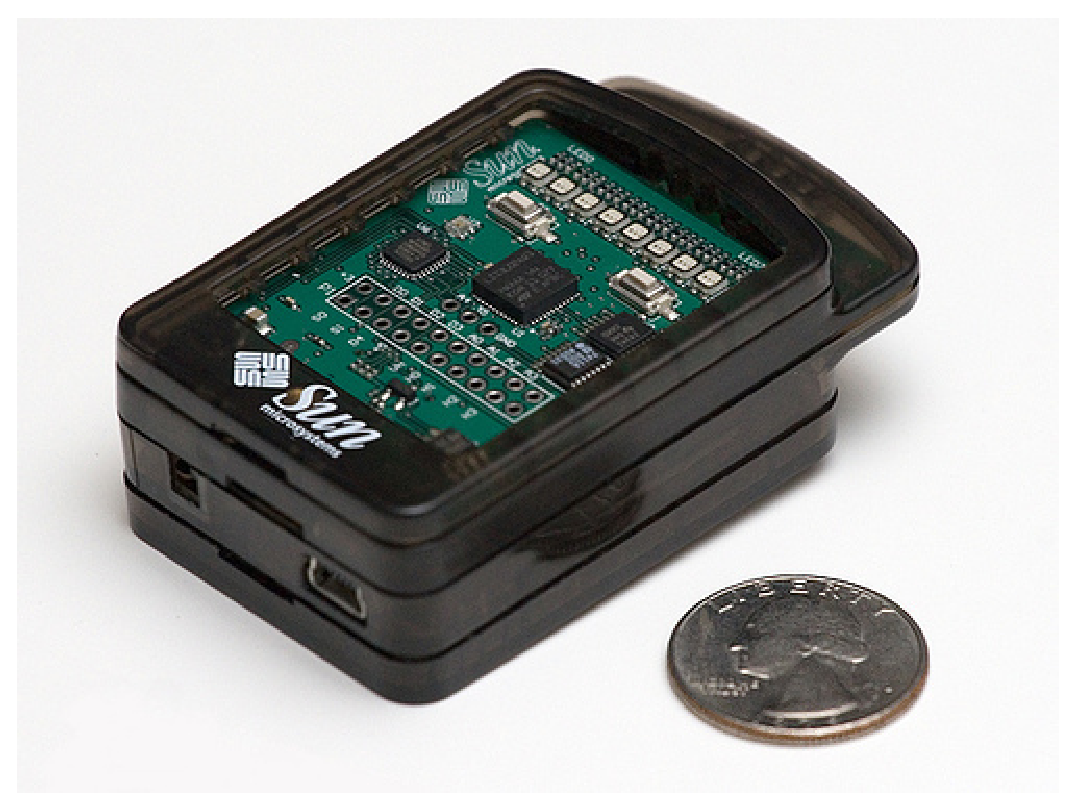
\includegraphics[scale=0.50]{img/sunspot1.eps} 
\caption[Sun SPOT device]{Sun SPOT device}
\label{Fig:SunSpot}
\end{figure} 


\subsection{The Squawk JVM}

The Squawk JVM is used on Sun SPOTs to enable on-board execution of Java
programs. The Squawk VM was originally developed for a smart card system with
even greater memory constraints than the Sun SPOTs. The Squawk JVM has the
following features \cite{simon_squawk:2006}:

\begin{itemize}
  \item It is written in Java, and specifically designed for resource
  constrained devices, meeting the requirements of Connected Limited Device
  Configuration 1.1 (CLDC) framework for Java Micro Edition (Java ME)
  applications.
  \item It does not require an underlying OS as it runs directly on the Sun
  SPOT hardware. This allows for a reduction in memory consumption.
  \item It suuports inter-device application migration.
  \item It allows the execution of multiple applications on one VM,
  representing each one as an object.
\end{itemize}

\subsection{Split VM Architecture}

As resource constrained devices are incapable of loading class files on-device
by virtue of their limited memory, a VM architecture known as the ``split VM
architecture'' is used, as shown in Figure
\ref{Fig:SquawkVM_architecture}.

\begin{figure}[h]
\centering
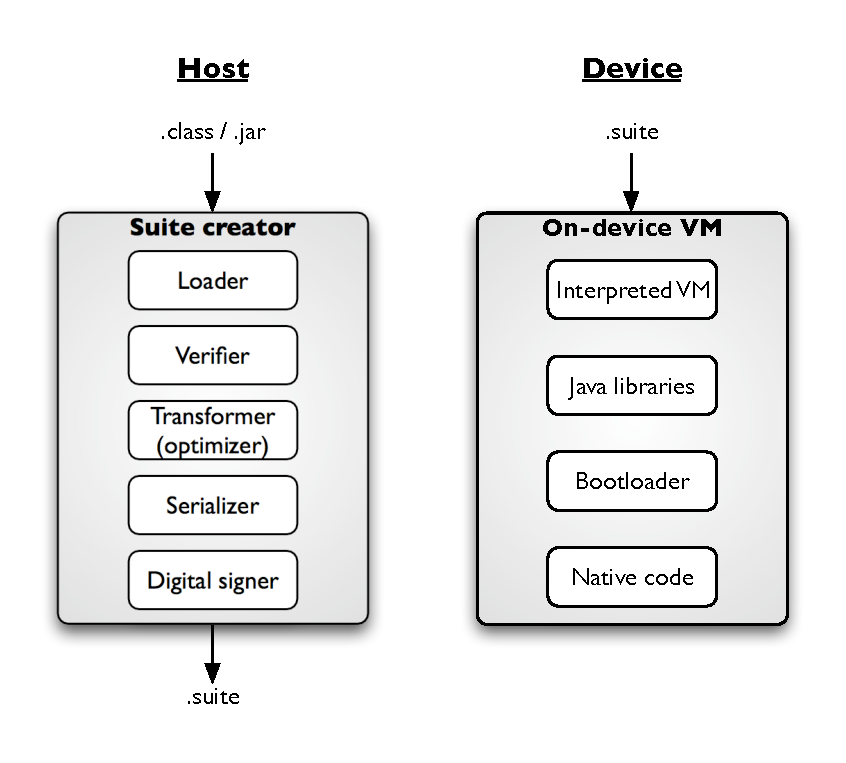
\includegraphics[scale=0.61]{img/Squawk_architecture.eps} 
\caption[The Squawk Split VM Architecture]{The Squawk
Split VM Architecture (reproduced from \cite{simon_squawk:2006})}
\label{Fig:SquawkVM_architecture}
\end{figure}  

The Squawk split VM architecture uses a class file preprocessor known as the
\emph{suite creator} that converts the \emph{.class} bytecode into a more
compact representation called the Squawk bytecode. According to
\cite{simon_squawk:2006}, Squawk bytecodes are optimised in order to:
\begin{itemize}
\item minimise space used by using smaller bytecode representation, escape
mechanisms for float and double instructions, and widened operands. 
\item enable in-place execution, by ``resolving symbolic references to other
classes, data members, and member functions into direct pointers, object offsets
and method table offsets respectively''.
\item simplify garbage collection, by the careful reallocation of local
variables, and by storing on the operand stack the operands of only those instructions that would result in a memory allocation.
\end{itemize}

The Squawk bytecodes are converted into a \emph{.suite} file created by
serialising and saving into a file the internal object memory representation.
These files are loaded on to the device, and subsequently interpreted by the
on-device VM.

\subsection{Sun SPOT applications} \label{subsec:sunspotapps}

Sun SPOT applications are divided into two classes:
\cite{sun_developer:2008}:

\begin{itemize}
  \item \emph{On-SPOT applications}
  \item \emph{On-Host applications}
\end{itemize}

\begin{figure}[h]
\centering
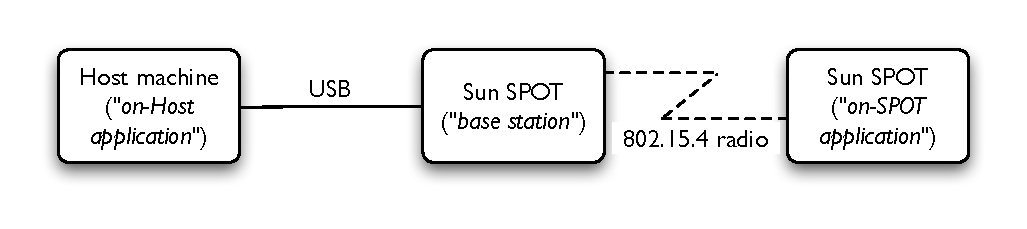
\includegraphics[width=\textwidth]{img/SunSPOTS_applications.eps} 
\caption[Types of Sun SPOT applications]{Types of Sun SPOT applications (adapted from
\cite{sun_developer:2008})}
\label{Fig:SunSPOTS_applications}
\end{figure}  

\emph{On-SPOT applications}  are deployed and
executed on a remote Sun SPOT that communicates untethered. On-SPOT
applications are Java programs that runs on the Squawk VM, and is compliant
with CLDC 1.1 specification. 

\emph{On-Host applications} run on the host machine
(typically a PC), and communicate with the network of Sun SPOTs through a base
station node that serves no purpose other than to facilitate Sun SPOT-host
machine communication. 
  
The base station node, which is a Sun SPOT itself, communicates with other
nodes in the network using RF communication, and with the host machine via a
USB link (see Figure \ref{Fig:SunSPOTS_applications}). The host application is
a Java 2 Standard Edition (J2SE) program.
  
 
\section{Summary}

This chapter presented an overview of the concepts, technologies, and hardware
underlying the work presented in this thesis. After underlining the need for the
use of programming models to increase the ubiquity of WSN use, this chapter
introduced a taxonomy of programming abstractions and placed the Distributed
Abstract Data Types programming abstraction used in this work within the
framework of the taxonomy. This was followed by a detailed discussion on Abstract
and Distributed Abstract Data Types used in the application layer of the
prototype produced during the course of this work, and the Logical Neighbourhood
routing mechanism used in the network and data link layers of the prototype. The
chapter concluded with a brief presentation of the SunSPOTs hardware platform,
and its particular suitability for the application under consideration. 


  
\chapter{Implementation} \label{chap:Implementation}

\begin{figure}
\centering
\label{Fig:DADTLN_architecture}
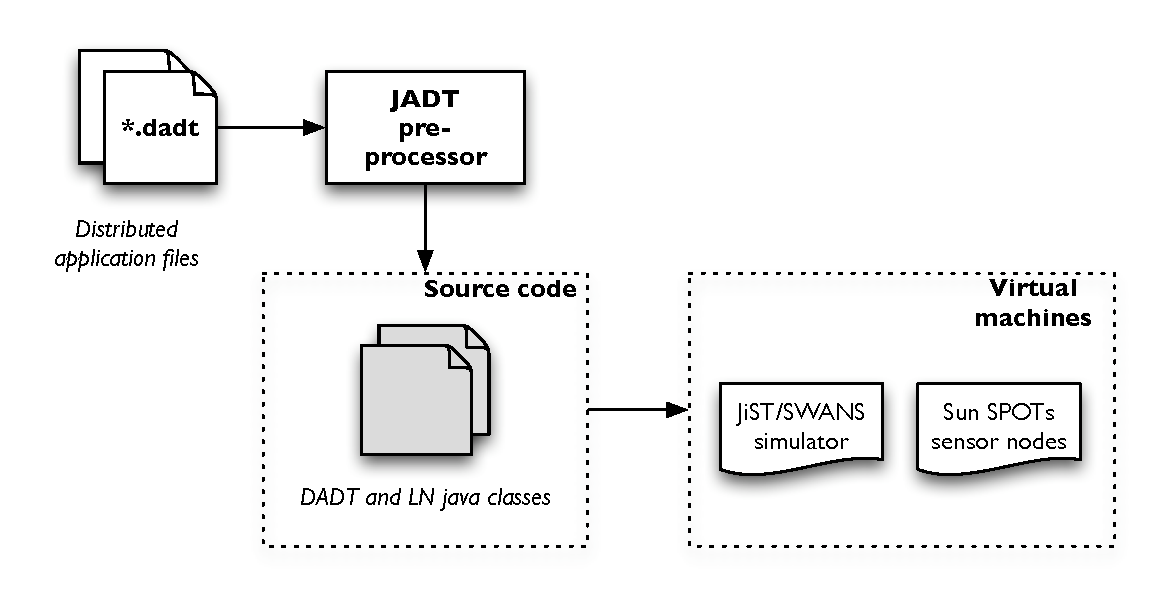
\includegraphics[scale=0.71]{img/DADTLN_architecture.eps} \caption[DADTLN
prototype architecture - to be renamed]{DADTLN prototype architecture - to
be moved to the other section}
\end{figure} 
\chapter{Evaluation} \label{chap:evaluation}

This chapter presents the results of the performance evaluation of the 
DADT/LN prototype running on real-world sensor nodes (Sun SPOTs). 

\section{Setting}

% Unless you already explained it somewhere else (and yet a reference to this
% "somewhere else" must be put in this chapter), the reader has very
%little information as to what your test application is doing. You need to give
%more details, say exactly what the application is supposed to accomplish and
%how.

The sample distributed application used for evaluation of the DADT/LN prototype 
implements an example WSN application where several sensor devices are deployed
in the environment and able to provide reports about some physical
phenomena, e.g. temperature. A monitoring station may access
particular sensor devices in WSN to aggregate their sensor readings, e.g. to
calculate average value, or reset sensors in case of problems.

The sample distributed application initially consists of the following files:
\begin{itemize}
  \item \emph{Sensor.java}, which defines the functionality of the device
  that provides sensing ability.
  \item \emph{SensorNode.dadt}, which defines the sensors and/or actuators available on the sensor
  device as abstract ADT instances, and binds them to the ``DSensor''  DADT type.
  \item \emph{ClientNode.dadt}, which is run by monitoring station
  in order to perform the distributed operation requests; the scope
  of the distributed operation is also declared here.
  \item \emph{DSensor.dadt}, which declares the list of available
  distributed operations, actions and properties.
\end{itemize}

As described in Section \ref{sec:PrototypeDesign}, the dadt files are translated
by DADT preprocessor into conventional java application. This
results into creation of additional java files, each of which represents DADT
Property and DADT Action classes (see Section \ref{subsec:DADTsConcepts}) that
were declared by application developer in \emph{DSensor.dadt} file. 

These files are named according the following naming scheme:
``DSensorXXXproperty'' or ``DSensorYYYaction'', where \emph{XXX} is a name of the
DADT Property and \emph{YYY} is a name of the DADT Action respectively. 

The functionality of the sample application is provided by the objects
of the runtime library of the DADT/LN prototype \ref{ADDREF}.  

The code of the distributed application is coupled with the
compiled runtime library to create 2 jar-files representing distributed
applications, namely the SensorNode and ClientNode applications, which were
deployed on the Sun SPOT devices.

6 Sun SPOT devices that form a simple WSN were used as a testbed for performing
their evaluation. Each of the Sun SPOT devices ran one of the LN/DADT prototype
distributed applications (ClientNode or SensorNode) application, as can be seen
in Figure \ref{Fig:EvaluationConfig}.

\begin{figure}
\centering
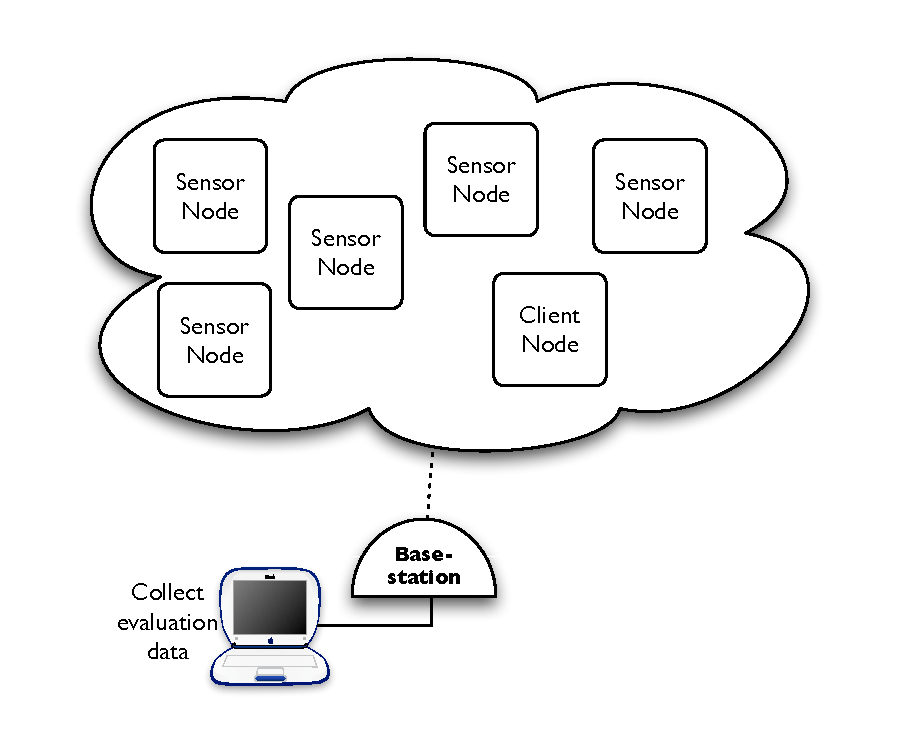
\includegraphics[scale=0.50]{img/EvaluationConfig.eps} 
\caption[Test-bed model of WSN using the DADT/LN prototype]{Test-bed model of WSN using the DADT/LN prototype}
\label{Fig:EvaluationConfig}
\end{figure}

The sensor device that ran the SensorNode application used the temperature and
light sensors available on the Sun SPOT demo sensor board. The DADT/LN prototype
on the sensor device abstracted those sensors using ADT instances, and provided
functionality to perform sensing and resetting operations. Communication between
sensor devices was supported by the LN implementation.

The sensor device that runs the ClientNode application was programmed to 
calculate the average temperature or luminosity value sensed by the set of
nodes. This set of nodes was specified implicitly using a DADT Dataview object
(see Section \ref{subsubsec:views}).


\section{Metrics}

The DADT/LN prototype was evaluated using the following metrics:
\begin{itemize}
\item Memory usage
\item Processing and communication delays
\end{itemize} 

These metrics were selected due to the fact that they allow to  ..  

%Here you need to "define" the various metrics, say what they are and so on...
%More importantly, however, you need to say *why* you picked these metrics and
%why they are important, which you completely miss right now. For instance,
%memory usage is important to measure because it determines how complex your
%application can be while still fitting in the node's memory. Delays are
%important to measure because they determine how scalable is the solution
%w.r.t. the number of DADT properties involved, number of devices in the
%network and so on... For each metric, you also need to say how you measured
%it. For instance, how did you measure the delays? Did you somewhat instrument
%the code?

\section{Results}

\subsection{Memory Usage}

As mentioned above, the memory requirements of the DADT/LN implementation are
based on the following components:
\begin{itemize}
  \item Distributed application code translated and compiled from dadt files
  \item The runtime library of the DADT/LN prototype
\end{itemize}



Table \ref{Tab:Memory} presents the memory requirements for the evaluated sample
distributed application.

\begin{table}

	\begin{center}
	\begin{tabular}{| p{1.8cm} | p{1.8cm} | p{1.8cm} |}
	\hline
	
	%There are free tools online to gather various statistics on source code
	% (WINDOWS), e.g., http://sourcecount.com/
	Filename & DADT Source code, bytes  & Java source code, Num of
	code lines Java bytecode size, bytes \\ \hline 
	
	Sensor.java & -  & tbc  3164 \\ \hline
	SensorNode.dadt \T \B & 477 \T \B & tbc \T \B tbc \\ \hline
	ClientNode.dadt \T \B & 841 \T \B & tbc \T \B tbc \\ \hline
	DSensor.dadt \T \B & 303 \T \B & tbc \T \B tbc \\ \hline
	\end{tabular}
	\end{center}
	\caption{Memory usage}
	\label{Tab:Memory}
\end{table}

As discussed before, the runtime library consists of a number
of Java files that provide the functionality of the DADT/LN prototype. The \emph{jar} file representing the runtime
library for the SUN SPOT device requires 81KB of memory. 

The runtime library was later integrated with the SensorNode application code 
resulting in 95KB jar-file. Similarly, the integrated jar-file of the ClientNode
application requires 99 KB of the memory.

\subsection{Processing and Communication Delays}

This section presents evaluation of the round trip delay time required for
executing a distributed sensing operation on the WSN.  

%%

The processing and communication delays were used to compare the performance of
the DADT/LN prototype upon execution of the distributed operation ``average''
over several such Dataviews. %rewrite%

The Dataview used to define the scope of the given distributed operation would be classified as follows:
\begin{itemize}
\item \emph{low} complexity, which consists of up to 3 DADT properties allowing to define
views, such as ``all active temperature sensors'';
\item \emph{moderate} complexity, which uses from 3 to 10 properties that allows to
create views, such as ``all active temperature
sensors with precision > 1.0 and sensor reading greater than 80'';
\item \emph{high} complexity, which uses up to 20 properties. The number of properties that construct such type of Dataviews was
limited by the length of the radiogram size used for communication between Sun SPOTs.
\end{itemize}

\begin{figure}
\centering
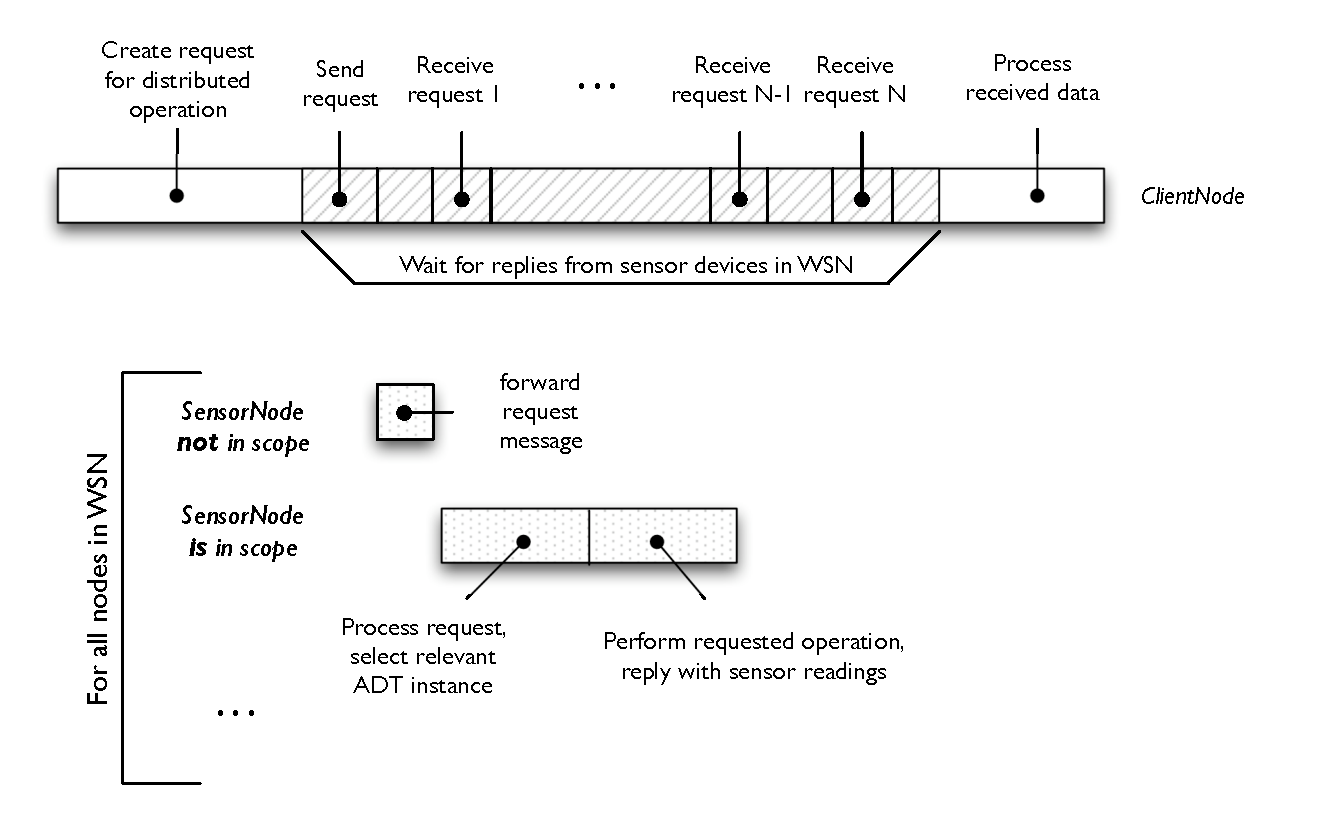
\includegraphics[scale=0.60]{img/RTTevaluation.eps} 
\caption[Delay factors for distributed operation execution]{Factors contributing to delays in the execution of a distributed operation on a WSN using the DADT/LN prototype}
\label{Fig:TimingsModel}
\end{figure}

Figure \ref{Fig:TimingsModel} shows the relevant time delays occurred during the
work of DADT/LN prototype. 

\subsubsection{Non-concurrent requests}

This section provides results of the evaluation of the average time intervals on the basis of single non-concurrent requests.

\begin{table}[h]
\begin{tabular*}{0.85\textwidth}{| p{1.8cm} | p{1.9cm} | p{2.1cm} | p{1.8cm} |
p{1.9cm} | p{1.9cm} | }
\cline{1-6} & \multicolumn{3}{|c|}{ClientNode Application} & \multicolumn{2}{|
c |}{SensorNode Application} \\ \cline{1-6}
Dataview complexity \T \B & Create request (ms) & Send request over LN and wait
for replies (ms) & Process sensor readings (ms) & Receive request, select ADT
instances & Perform requested action and send reply \\ \cline{1-6}
Low & 44.64 & 1414.27 & 203.91 & 520.13 & 92.94  \\ \cline{1-6}
Moderate & 49.82 & 3101.91 & 203.45 & 943.02 & 93.76 \\ \cline{1-6}
High  & 62.55 & 6034.82 & 205.45 & 1077.83 & 89.95 \\ \cline{1-6}
\end{tabular*}
\caption{Processing and communication delays for non-concurrent requests for
execution of distributed operation ``average''}
\label{Tab:EvalRes}
\end{table}

As can be seen in Table \ref{Tab:EvalRes}, the complexity of the 
Dataview has a direct correlation to the delays associated with processing of the request
on the SensorNode side. This subsequently leads to increasing waiting
intervals on the ClientNode side.

On the SensorNode, this might be a consequence of the given limitations of the
Squawk JVM, which does not provide support for serialization of objects. Hence,
delays occur when the object representing the scope of the distributed operation is
recreated by the SensorNode, and is later used for identifying the relevant ADT
instances which execute the requested operation.
Activities such as performing an action that involve: (a) requesting sensor
readings, and (b) the subsequent invocation of the LN API to send a reply message, were
executed in a relatively short time.

On the ClientNode, actions such as preparing a request message and parsing
the received results take on average 10-15\% of the time spent waiting for the receipt of reply messages with sensor readings.

\subsubsection{Concurrent requests}

Table \ref{Tab:EvalResConcurrent} shows the processing time delays caused by
concurrent requests on the WSN. The WSN used as part of this evaluation consisted
of two devices running the Client Node application, which issued concurrent
distributed operation execution requests. 
Evaluation of the concurrent requests was based on the assumption that these
requests may be 10-80 ms apart in time.

\begin{table}[h]
\begin{tabular*}{0.85\textwidth}{| p{1.8cm} | p{1.9cm} | p{2.1cm} | p{1.8cm} |
p{1.9cm} | p{1.9cm} | }
\multicolumn{3}{|c|}{ClientNode Application} & \multicolumn{2}{|
c |}{SensorNode Application} \\ \cline{1-6}
Dataview complexity & Create request, ms & Send request over LN and wait
for replies, ms & Process sensor readings, ms & Receive request, select ADT
instances & Perform requested action and send reply \\ \cline{1-6}
Low & 51.40 & 2604.75 & 197.85 & 595.95 & 178.84  \\ \cline{1-6}
\end{tabular*}
\caption{Processing and communication delays for concurrent requests for
execution of distributed operation ``average''}
\label{Tab:EvalResConcurrent}
\end{table}

The results presented in Table \ref{Tab:EvalResConcurrent} considered only those
Dataviews with low complexity. For concurrent requests over Dataviews with a
high-level of complexity, the time delays were found to be inappropriately large
for executing a distributed operation.

It can be seen that, in general, concurrent requests increase the processing time
on devices running the SensorNode application. However, the other delay factors
involved in the execution of the distributed operation are comparable to that
incurred upon execution of non-concurrent requests.

%%% SUGGESTION: PLACE IN SEPARATE SECTION %%
Future work may include further evaluation and adaptation of the DADT/LN
prototype to provide acceptable performance for Dataviews of moderate and high complexity
containing of a large number of DADT properties. 




\chapter{Evaluation, Conclusions, and Future Work} \label{chap: Evaluation}
 \section{Evaluation}

The metric used to evaluate the performance of the DADT/LN prototype is
the packet processing workload on the application layer. This metric was used to
compare the performance of the DADT/LN prototype against that of the original
DADT prototype used as the basis for this work \cite{migliavacca_DADT:2006}. 

In the original DADT prototype, a request message
was either replied to or discarded by the application layer entity on the basis of the
evaluation of an abstract tree representing the specified scope of the operation. In
the implementation presented in this work, the integration with the LN approach
results in unsuitable request messages being discarded on the basis of predicate
evaluation in the network layer.

//add the graph here

A series of simulations were run using the JiST/SWANS simulator to determine
the number of request messages discarded in the network layer, and the number
passed on to the application layer by the LN predicate matching algorithm. 
It was found that for every distributed operation request that was limited in
scope to a set of ADT instances present only in a subset of the sensor nodes in
the network, the number of packets forwarded to the DADT/LN prototype's
application layer for processing was lower than the corresponding number in the
original DADT prototype. In the worst case scenario where every sensor node in
the network has at least one ADT instance that falls within the scope of the
operation, the application layer traffic on both prototypes is the same.

\section{Conclusions}

During the course of this project, it was proven that the concept of DADTs can be
applied to real world WSNs. The proof-of-concept prototype implemented indicates
the potential of programming abstractions in helping reduce the effort involved
in developing applications for WSNs.
In addition, upon integrating the innovative LN routing mechanism
with the DADT implementation on the application layer, there was found to be a
significant reduction in the amount of processing performed in the application
layer. 
 
\section{Future Work}

This section presents a list of possible extensions to the work implemented as
part of this thesis. These include:

\begin{itemize}
  \item \emph{Support for DADT selection operators:} The current prototype
  supports the selection of all ADT instances that match a defined DADT Data
  view, but does not enable the selection of a subset of the aforementioned
  collection of ADT instances. This arises from the limitations of the current
  LN implementation.
  \item \emph{Extending support for Space DADTs:} Currently, the prototype
  provides a limited support for the notion of space. Therefore, a possible
  avenue for future work could include the full support for Space DADTs
  provided by the prototype.
  \item \emph{Extending the prototype for networks of heterogenous nodes:}
  The current prototype, by virtue of it being implemented in Java, cannot be
  used on a wide variety of different nodes. 
\end{itemize}


\bibliography{references}
\bibliographystyle{acm}


\end{document}
